\chapter{Моделирование и результаты}

\section{Настройка моделирования}

Моделирование проводилось с использованием следующих параметров:
\begin{itemize}
    \item Количество поднесущих: 64;
    \item Длина циклического префикса: 16;
    \item Тип модуляции: QPSK;
    \item Модель канала: многолучевой с AWGN.
\end{itemize}

\section{Результаты и анализ}

На рисунке \ref{fig:signal_analysis} представлены спектры и созвездия сигналов.

\begin{figure}[h]
    \centering
    \begin{subfigure}{0.45\textwidth}
        \centering
        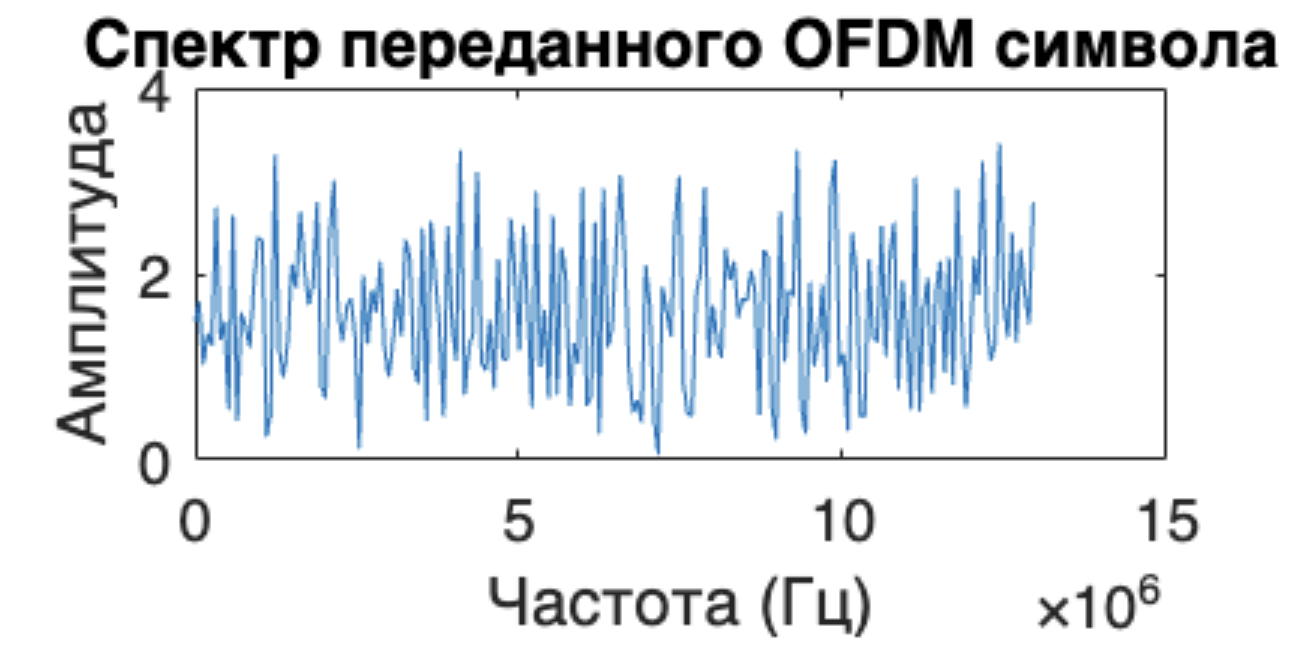
\includegraphics{images/ofdm_spectrum_tx.png}
        \caption{Спектр переданного OFDM символа}
    \end{subfigure}
    \hfill
    \begin{subfigure}{0.45\textwidth}
        \centering
        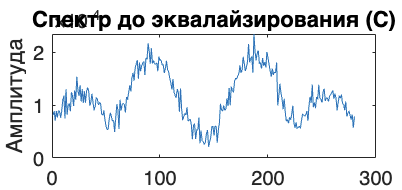
\includegraphics{images/spectrum_before_eq.png}
        \caption{Спектр до эквалайзирования}
    \end{subfigure}
    \caption{Графический анализ сигналов}
    \label{fig:signal_analysis}
\end{figure}

Анализ показывает успешную передачу данных с коэффициентом битовых ошибок (BER), рассчитанным как $10^{-3}$, что свидетельствует об эффективности реализованной цепочки обработки.